\section{Verdrängungsstrategie}
\textcolor{myblue}{FIFO}: Entferne jeweils älteste Page. Problem: alte, aber häufig benutzte Pages werden gleich wieder geladen.\\
\textcolor{myblue}{Second Chance (Extension FIFO)}: Pages erhalten ein A(ccess)-Bit und es wird
jeweils die älteste, nicht verwendete Page entfernt. Verliert eine Page ein "Leben" rutscht sie ganz an den Anfang. Bekommt eine Page ein "Leben" bleibt es an der Stelle (links alt, rechts neu).\\
\textcolor{myblue}{Optimal}: Ersetze die Page, die in Zukunft am spätesten verwendet wird (nicht umsetzbar, da man nicht weiss welche diese sind)\\
\textcolor{myblue}{LRU (Least recently used)}: Ersetzt, die am längsten unbenutzte Page.Bei jedem Zugriff wird ein Timestamp gesetzt, Page mit kleinstem T wird ersetzt. (Nahe am Optimum)\\
\textcolor{myblue}{NFU (not frequently used)}: Benötigt Counter Table pro Page Table eine n-Counter am selben Index. OS zählt Intervalle, in denen es Zugriffe gab.\\
\textbf{Problem}: Auch alte Pages können lange bestehen bleiben, wenn sie zu Beginn sehr oft verwendet wurden.\\
\textcolor{myblue}{NFU mit Aging}: Die Counter werden neu auch nach Zeit gewichtet.
\subsection{Buddy-System}
Das Buddy-System teilt Prozessen Speicher zu. Der Speicher wird in 2 k Bereiche aufgeteilt und zu Beginn gibt es einen Block, der möglichst den gesamten Speicher abdeckt. Falls Speicher nicht als Zweierpotenz ausgedrückt werden kann, dann kann er auch als mehrere Blöcke unterschiedlicher Grössen unterteilt werden. Wenn es keinen Block in der Grösse gibt, dann wird die nächstgrössere 2-er-Potenz genommen. Terminieren Prozesse, dann erkennt das System die Buddies wieder und fügt die Partitionen zusammen. Wird fürs Paging aktueller Betriebssysteme verwendet.
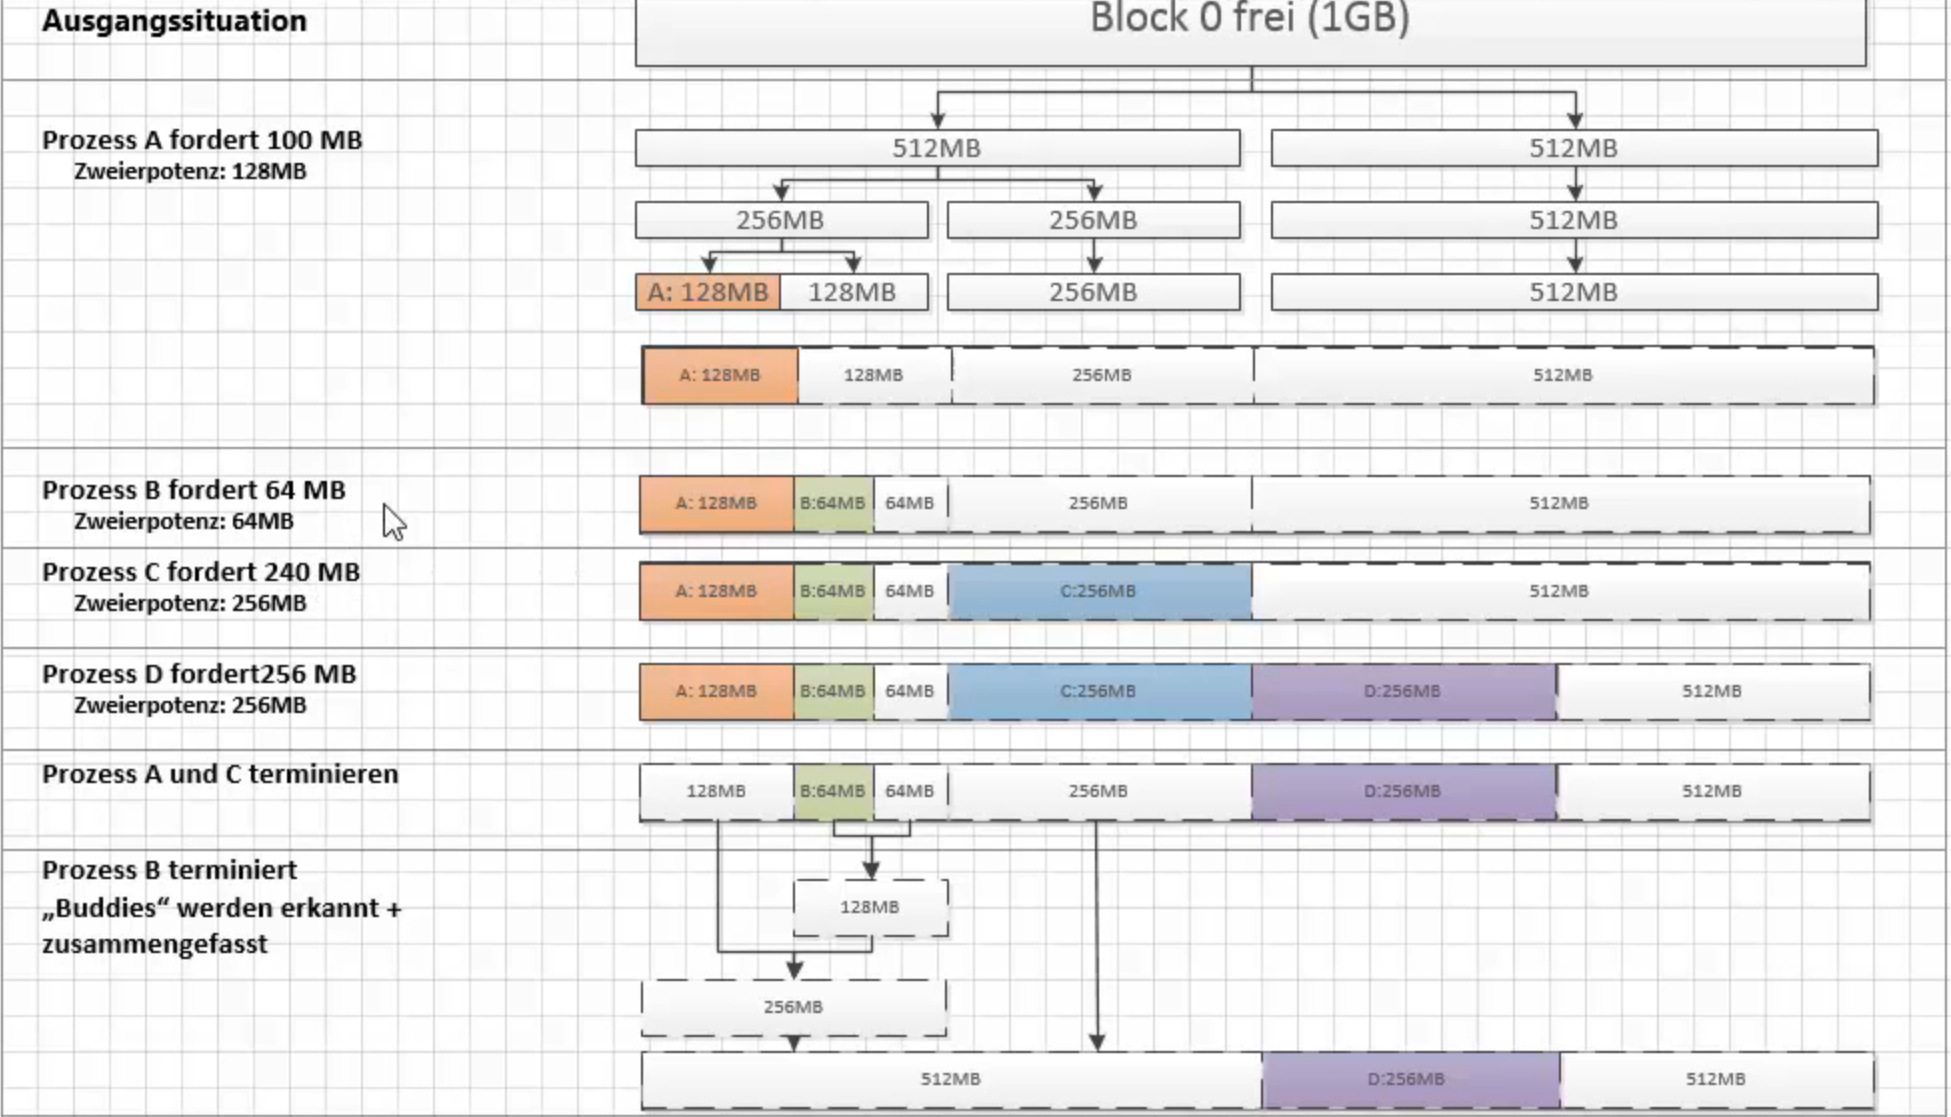
\includegraphics[width=\columnwidth]{buddy_system.png}
\subsection{Berechnungen}
Bei 16MB virtueller Adressraum, 4KB Pages, 64KB Hauptspeicher, Single Level:\\
\textcolor{myblue}{Anzahl Bits für virtuelle Adresse} $2^{24} \rightarrow 24 Bit$\\
\textcolor{myblue}{Grösste virtuelle Adresse} $FFFFFF_h = 2^{24} - 1$\\
\textcolor{myblue}{Kleinste virtuelle Adresse}: $000000 h$\\
\textcolor{myblue}{Anzahl Bits für reale Adresse} $2^{16} \rightarrow 16 Bit$\\
\textcolor{myblue}{Grösste physische Adresse}: $FFFF_h = 2^{16} - 1$\\
\textcolor{myblue}{Kleinste physische Adresse}: $0000_h$\\
\textcolor{myblue}{Anzahl Pages}: Virtueller Adressraum, Grösse einer Page. Hier =$2^{12}$ Pages\\
\textcolor{myblue}{Anzahl Frames}: Hauptspeicher, Grösse gleich wie Pagegrösse. Hier = $16 Page$ Frames\\
\textcolor{myblue}{Offset}: Bei $4 KB$ Page $= 2^{12} = 12 Bit$ Offset\\
\textcolor{myblue}{Grösse Framenummer}: Ist der Teil der realen Adresse ohne den Offset. Hier $16 Bit$ ohne Offset ($12 Bit$) = $4 Bit$ für die Framenummer. Oder: Page Frames als 2-er-Potenz und der Exponent als Bit.
\textcolor{myblue}{Grösse einer Pagetable (ohne Statusbits)}: Anzahl Pages * Framenummer.\\\\
\textcolor{myblue}{Bestimmen einer Adresse}: $3AB4_h \rightarrow$ Pagenummer = $3 \rightarrow$ Offset = $AB4 \rightarrow$ reale Adresse hier $5AB4_h$ In diesem Bsp. liegen Pages 2 bis 5 in den Frames 4 bis 7. Bsp. Auf Frame 5 werden Adressen von $3000_h$ bis $3FFF_h$ abgebildet.
% 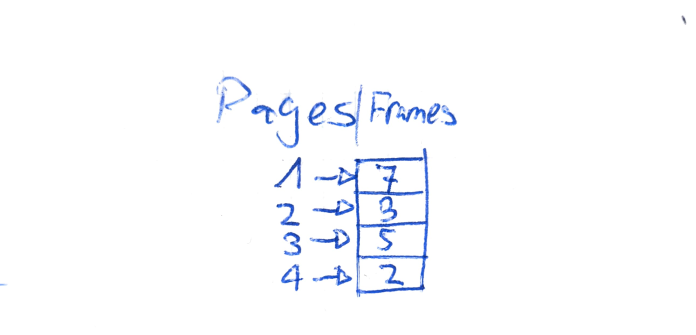
\includegraphics[width=\columnwidth]{address_definition.png}
% \vspace*{\fill}%